\documentclass[a4paper, czech]{article}

\usepackage[czech]{babel}
\usepackage{indentfirst}
\usepackage{graphicx}
\usepackage{float}
\usepackage[margin=1.5cm]{geometry}
\usepackage{booktabs}
\usepackage{amsmath}
\usepackage[dvipsnames, table]{xcolor}
\usepackage{multirow}
\usepackage{tabularray}
\usepackage{bold-extra}
\usepackage{circuitikz}
\usepackage{caption}
\usepackage{subcaption}
\usepackage[utf8]{inputenc}
\usepackage{array}
\usepackage{nicematrix}
\usepackage{gensymb}

\begin{document}
\begin{table}[H]
    \centering
    \begin{tblr}{
        cell{1}{1} = {c = 2, r = 4}{c}, % Logo
        cell{1}{4} = {c = 3}{c}, % Předmět
        cell{2}{4} = {c = 3}{c}, % Jméno
        cell{3}{4} = {}{c}, % Ročník
        cell{3}{6} = {}{c}, % Studijní skupina
        cell{4}{4} = {}{c}, % Spolupracoval
        cell{4}{6} = {}{c}, % Mereno dne
        cell{5}{1} = {c = 2}{55mm}, % Kontroloval
        cell{5}{3} = {c = 2}{55mm}, % Hodnoceni
        cell{5}{5} = {c = 2}{55mm}, % Dne
        cell{6}{2} = {c = 5}{}, % Nazev ulohy
        cell{7}{1} = {}{c}, % Číslo úlohy
        cell{7}{2} = {c = 5}{c}, % Název úlohy
        vline{1,2,7} = {1.2pt},
        vline{3,5},
        hline{1,5,6,8} = {1.2pt},
        hline{2,3,4}
        }
        
\includegraphics{logo_fekt.png} & & \textsuperscript{Předmět} & \large \textbf{Měření v audiotechnice} \\
             & & \textsuperscript{Jméno} & \large \textbf{Karolína Šebestová} \\
             & & \textsuperscript{Ročník} & \large \textbf{3.} & \textsuperscript{Studijní skupina} & \large \textbf{St 14:00} \\
             & & \textsuperscript{Spolupracoval} & \large \textbf{Filip Kokavec} & \textsuperscript{Měřeno dne} & \large \textbf{27.11.2024} \\
        \textsuperscript{Kontroloval} & & \textsuperscript{Hodnocení} & & \textsuperscript{Dne} \\
        \textsuperscript{Číslo úlohy} & \textsuperscript{Název úlohy} \\
        \Large \textbf{9B} & \Large \textsc{\textbf{Měření kmitočtové závislosti impedance cívky}} \\
    \end{tblr}
\end{table}

\section{Zadání}

\begin{itemize}
    \item Změřte kmitočtovou závislost indukčnosti a činitele jakosti dvou téměř identických
    cívek pro audiotechniku. Jeden přípravek obsahuje cívku s feritovým jádrem, druhý
    bez jádra.
    \item Změřte kmitočtovou závislost impedance cívky s jádrem a bez jádra.
    \item Porovnejte možnosti měření impedance cívky pomocí osciloskopu a metodou tří
    voltmetrů.
\end{itemize}

\section{Teoretický úvod}

\begin{figure}[H]
    \centering
    \begin{circuitikz}[european, straight voltages]
        \draw (0,0) node[draw, rectangle, align=center, line width=0.8, minimum height=1cm, inner xsep=7.5](trafo){Oddělovací\\transformátor}
        (trafo.east) ++(0,0.25) to ++(0.5,0)
        (trafo.east) ++(0,-0.25) to ++(0.5,0)
        (trafo.east) ++(0.5,0) node[draw, rectangle, anchor=west, align=center, line width=0.8, minimum height=1cm, inner xsep=7.5](generátor){Generátor}
        (generátor.east) ++(0,0.25) to ++(0.5,0) to ++(0,1.25) to ++(1,0) node[circ](uzel1){}
        to[rmeter, t=V, v=$U$] ++(0,-3) node[circ]{}
        (uzel1) to ++(1.5,0) node[circ, label=Kanál 1](uzel2){} to[rmeter, t=osc, name=osc] ++(0,-3) node[circ, label=below:Kanál 2]{}
        (uzel2) to ++(1.5,0) node[circ](uzel3){} to[rmeter, t=V$_Z$] ++(0,-1.5) node[circ](uzel4){}
        to[rmeter, t=V$_R$] ++(0,-1.5) node[circ]{}
        (uzel4) to (osc.north)
        (uzel3) to ++(1.5,0) node[ocirc, scale=1.5](svorka1){}
        (uzel4) to ++(1.5,0) node[ocirc, scale=1.5](svorka2){} to ++(1.5,0) node[circ](uzel5){}
        (svorka1) to ++(1.5,0) to[cute choke, label=L$_\text{X}$, v=$U_Z$] (uzel5)
        (uzel5) to[R, label=R, v<=$U_R$] ++(0,-1.5) to ++(-1.5,0) node[ocirc, scale=1.5](svorka3){} to ++(-5.5,0)
        to ++(0,1.25) to ++(-0.5,0)
        (uzel5) to ++(0.75,0) node[rground]{};
        \draw[dashed, line width=1.2] (svorka1) -- (svorka2) -- (svorka3) -- ++(0,-0.2)
        to node[below]{Měřený přípravek} ++(3,0) -- ++(0,3.4) -- ++(-3,0) -- (svorka1);
        \draw (svorka1) node[above left]{1}
        (svorka2) node[above left]{2}
        (svorka3) node[above left]{3};
    \end{circuitikz}
    \caption{Zapojení pro měření kmitočtové závislosti cívky}
\end{figure}

\section{Výsledky měření}

\subsection{Tabulky}

\begin{table}[H]
    \catcode`\-=12
    \centering
    \caption{Měření kmitočtové závislosti cívky metodou tří voltmetrů - \textbf{cívka bez jádra}}
    \begin{NiceTabular}{rccc>{\columncolor{gray!15}}c>{\columncolor{gray!15}}c>{\columncolor{gray!15}}c>{\columncolor{gray!15}}c>{\columncolor{gray!15}}c>{\columncolor{gray!15}}c>{\columncolor{gray!15}}c}
        \toprule
        \multicolumn{1}{c}{$f$}      & $U_\text{R}$   & $U_\text{Z}$    & $U$    & $Z$     & $\varphi$     & $R_\text{S}$    & $L_\text{S}$    & $R_\text{P}$    & $L_\text{P}$    & $Q$     \\
        \cmidrule(rl){1-1}
        \cmidrule(rl){2-2}
        \cmidrule(rl){3-3}
        \cmidrule(rl){4-4}
        \cmidrule(rl){5-5}
        \cmidrule(rl){6-6}
        \cmidrule(rl){7-7}
        \cmidrule(rl){8-8}
        \cmidrule(rl){9-9}
        \cmidrule(rl){10-10}
        \cmidrule(rl){11-11}
        \multicolumn{1}{c}{Hz}     & mV   & mV    & mV   & $\Omega$     & $\degree$     & $\Omega$     & mH    & $\Omega$     & mH    & -     \\
        \midrule
        20     & 1\,000 & 13,6  & 1\,010 & 1,36  & 42,93 & 0,996 & 7,371 & 1,857 & 15,89 & 0,930 \\
        50     & 1\,000 & 13,7  & 1\,011 & 1,37  & 36,82 & 1,097 & 2,614 & 1,711 & 7,276 & 0,749 \\
        100    & 1\,000 & 14,6  & 1\,012 & 1,46  & 34,96 & 1,197 & 1,331 & 1,781 & 4,055 & 0,699 \\
        200    & 1\,000 & 17,7  & 1\,014 & 1,77  & 38,03 & 1,394 & 0,868 & 2,247 & 2,286 & 0,782 \\
        500    & 1\,000 & 31,7  & 1\,014 & 3,17  & 64,60 & 1,360 & 0,912 & 7,391 & 1,117 & 2,106 \\
        1\,000  & 1\,000 & 59,3  & 1\,016 & 5,93  & 75,98 & 1,437 & 0,916 & 24,47 & 0,973 & 4,004 \\
        2\,000  & 1\,000 & 117,4 & 1\,024 & 11,74 & 81,48 & 1,740 & 0,924 & 79,23 & 0,945 & 6,674 \\
        5\,000  & 1\,000 & 295,8 & 1\,067 & 29,58 & 85,06 & 2,550 & 0,938 & 343,2 & 0,945 & 11,56 \\
        10\,000 & 1\,000 & 592   & 1\,197 & 59,2  & 86,01 & 4,117 & 0,940 & 851,2 & 0,944 & 14,34 \\
        15\,000 & 1\,000 & 893   & 1\,382 & 89,3  & 86,39 & 5,624 & 0,946 & 1418  & 0,949 & 15,85 \\
        20\,000 & 1\,000 & 1\,193  & 1\,606 & 119,3 & 86,25 & 7,799 & 0,947 & 1825  & 0,951 & 15,26 \\
        \bottomrule
    \end{NiceTabular}
\end{table}

\begin{table}[H]
    \catcode`\-=12
    \centering
    \caption{Měření kmitočtové závislosti cívky pomocí osciloskopu - \textbf{cívka s jádrem}}
    \begin{NiceTabular}{rcc>{\columncolor{gray!15}}cc>{\columncolor{gray!15}}c>{\columncolor{gray!15}}c>{\columncolor{gray!15}}c>{\columncolor{gray!15}}c>{\columncolor{gray!15}}c}
        \toprule
        \multicolumn{1}{c}{$f$}      & $I$   & $U_\text{Z}$ & $Z$     & $\varphi$     & $R_\text{S}$    & $L_\text{S}$    & $R_\text{P}$    & $L_\text{P}$    & $Q$     \\
        \cmidrule(rl){1-1}
        \cmidrule(rl){2-2}
        \cmidrule(rl){3-3}
        \cmidrule(rl){4-4}
        \cmidrule(rl){5-5}
        \cmidrule(rl){6-6}
        \cmidrule(rl){7-7}
        \cmidrule(rl){8-8}
        \cmidrule(rl){9-9}
        \cmidrule(rl){10-10}
        \multicolumn{1}{c}{Hz}     & mA   & mV & $\Omega$     & $\degree$     & $\Omega$     & mH    & $\Omega$     & mH    & -     \\
        \midrule
        20     & 9,932 & 13,74 & 1,374 & 5  & 1,369 & 0,953 & 1,379 & 125,4 & 0,087 \\
        50     & 9,889 & 13,94 & 1,394 & 12 & 1,364 & 0,923 & 1,425 & 21,35 & 0,213 \\
        100    & 9,881 & 14,79 & 1,479 & 24 & 1,351 & 0,957 & 1,619 & 5,787 & 0,445 \\
        200    & 9,885 & 18,02 & 1,802 & 40 & 1,380 & 0,922 & 2,352 & 2,231 & 0,839 \\
        500    & 9,900 & 32,76 & 3,276 & 66 & 1,332 & 0,953 & 8,054 & 1,141 & 2,246 \\
        1\,000  & 9,917 & 61,17 & 6,117 & 78 & 1,272 & 0,952 & 29,42 & 0,995 & 4,705 \\
        2\,000  & 9,967 & 119,5 & 11,95 & 83 & 1,457 & 0,944 & 98,07 & 0,958 & 8,144 \\
        5\,000  & 10,06 & 301,2 & 30,12 & 88 & 1,051 & 0,958 & 863,0 & 0,959 & 28,64 \\
        10\,000 & 10,07 & 603,5 & 60,35 & 88 & 2,106 & 0,960 & 1\,729  & 0,961 & 28,64 \\
        15\,000 & 10,03 & 898,6 & 89,86 & 88 & 3,136 & 0,953 & 2\,575  & 0,954 & 28,64 \\
        20\,000 & 9,969 & 1191  & 119,1 & 87 & 6,232 & 0,946 & 2\,275  & 0,949 & 19,08 \\
        \bottomrule
    \end{NiceTabular}
\end{table}

\begin{table}[H]
    \catcode`\-=12
    \centering
    \caption{Měření kmitočtové závislosti cívky metodou tří voltmetrů - \textbf{cívka s jádrem}}
    \begin{NiceTabular}{rccc>{\columncolor{gray!15}}c>{\columncolor{gray!15}}c>{\columncolor{gray!15}}c>{\columncolor{gray!15}}c>{\columncolor{gray!15}}c>{\columncolor{gray!15}}c>{\columncolor{gray!15}}c}
        \toprule
        \multicolumn{1}{c}{$f$}      & $U_\text{R}$   & $U_\text{Z}$    & $U$    & $Z$     & $\varphi$     & $R_\text{S}$    & $L_\text{S}$    & $R_\text{P}$    & $L_\text{P}$    & $Q$     \\
        \cmidrule(rl){1-1}
        \cmidrule(rl){2-2}
        \cmidrule(rl){3-3}
        \cmidrule(rl){4-4}
        \cmidrule(rl){5-5}
        \cmidrule(rl){6-6}
        \cmidrule(rl){7-7}
        \cmidrule(rl){8-8}
        \cmidrule(rl){9-9}
        \cmidrule(rl){10-10}
        \cmidrule(rl){11-11}
        \multicolumn{1}{c}{Hz}     & mV   & mV    & mV   & $\Omega$     & $\degree$     & $\Omega$     & mH    & $\Omega$     & mH    & -     \\
        \midrule
        20     & 1\,000 & 14,1  & 1\,012 & 1,41  & 31,88 & 1,197 & 5,927 & 1,661 & 21,24 & 0,622 \\
        50     & 1\,000 & 16,9  & 1\,013 & 1,69  & 40,02 & 1,294 & 3,460 & 2,207 & 8,365 & 0,840 \\
        100    & 1\,000 & 25    & 1\,014 & 2,5   & 56,54 & 1,379 & 3,319 & 4,534 & 4,770 & 1,513 \\
        200    & 1\,000 & 44,3  & 1\,014 & 4,43  & 72,78 & 1,312 & 3,367 & 14,96 & 3,691 & 3,226 \\
        500    & 1\,000 & 106,6 & 1\,019 & 10,66 & 82,73 & 1,350 & 3,366 & 84,18 & 3,421 & 7,833 \\
        1\,000  & 1\,000 & 211,7 & 1\,037 & 21,17 & 85,86 & 1,528 & 3,361 & 293,4 & 3,378 & 13,82 \\
        2\,000  & 1\,000 & 421   & 1\,106 & 42,1  & 86,87 & 2,300 & 3,345 & 770,7 & 3,355 & 18,28 \\
        5\,000  & 1\,000 & 1064  & 1\,486 & 106,4 & 87,95 & 3,805 & 3,385 & 2\,975  & 3,389 & 27,95 \\
        10\,000 & 1\,000 & 2139  & 2\,393 & 213,9 & 87,98 & 7,556 & 3,402 & 6\,055  & 3,406 & 28,29 \\
        15\,000 & 1\,000 & 3222  & 3\,405 & 322,2 & 88,11 & 10,64 & 3,417 & 9\,760  & 3,421 & 30,27 \\
        20\,000 & 1\,000 & 4240  & 4\,390 & 424   & 88,01 & 14,72 & 3,372 & 12\,209 & 3,376 & 28,78 \\
        \bottomrule
    \end{NiceTabular}
\end{table}

\begin{table}[H]
    \catcode`\-=12
    \centering
    \caption{Měření kmitočtové závislosti cívky pomocí osciloskopu - \textbf{cívka bez jádra}}
    \begin{NiceTabular}{rcc>{\columncolor{gray!15}}cc>{\columncolor{gray!15}}c>{\columncolor{gray!15}}c>{\columncolor{gray!15}}c>{\columncolor{gray!15}}c>{\columncolor{gray!15}}c}
        \toprule
        \multicolumn{1}{c}{$f$}      & $I$   & $U_\text{Z}$ & $Z$     & $\varphi$     & $R_\text{S}$    & $L_\text{S}$    & $R_\text{P}$    & $L_\text{P}$    & $Q$     \\
        \cmidrule(rl){1-1}
        \cmidrule(rl){2-2}
        \cmidrule(rl){3-3}
        \cmidrule(rl){4-4}
        \cmidrule(rl){5-5}
        \cmidrule(rl){6-6}
        \cmidrule(rl){7-7}
        \cmidrule(rl){8-8}
        \cmidrule(rl){9-9}
        \cmidrule(rl){10-10}
        \multicolumn{1}{c}{Hz}     & mA   & mV & $\Omega$     & $\degree$     & $\Omega$     & mH    & $\Omega$     & mH    & -     \\
        \midrule
        20     & 9,938 & 14,29 & 1,429  & 16,7 & 1,368 & 3,267 & 1,491  & 39,56 & 0,300 \\
        50     & 9,879 & 17,18 & 1,718  & 38   & 1,354 & 3,367 & 2,180  & 8,883 & 0,781 \\
        100    & 9,882 & 25,07 & 2,507  & 58   & 1,328 & 3,383 & 4,731  & 4,705 & 1,600 \\
        200    & 9,885 & 44,53 & 4,453  & 73   & 1,302 & 3,389 & 15,23 & 3,705 & 3,271 \\
        500    & 9,893 & 106,0 & 10,59 & 83   & 1,291 & 3,347 & 86,94  & 3,398 & 8,144 \\
        1\,000  & 9,911 & 210,7 & 21,06 & 86   & 1,470 & 3,345 & 302,0 & 3,361 & 14,30 \\
        2\,000  & 9,958 & 424,8 & 42,48  & 89   & 0,741 & 3,380 & 2\,434 & 3,381 & 57,29 \\
        5\,000  & 10,06 & 1\,072  & 107,2 & 89   & 1,871 & 3,412 & 6\,143   & 3,413 & 57,29 \\
        10\,000 & 10,07 & 2\,163  & 216,2 & 89   & 3,775 & 3,442 & 12\,393  & 3,443 & 57,29 \\
        15\,000 & 10,02 & 3\,213  & 321,2 & 89   & 5,607 & 3,408 & 18\,409  & 3,409 & 57,29 \\
        20\,000 & 9,972 & 4\,284  & 428,4 & 89   & 7,477 & 3,409 & 24\,548  & 3,410 & 57,29 \\
        \bottomrule
    \end{NiceTabular}
\end{table}

\subsection{Grafy}

\begin{figure}[H]
    \centering
    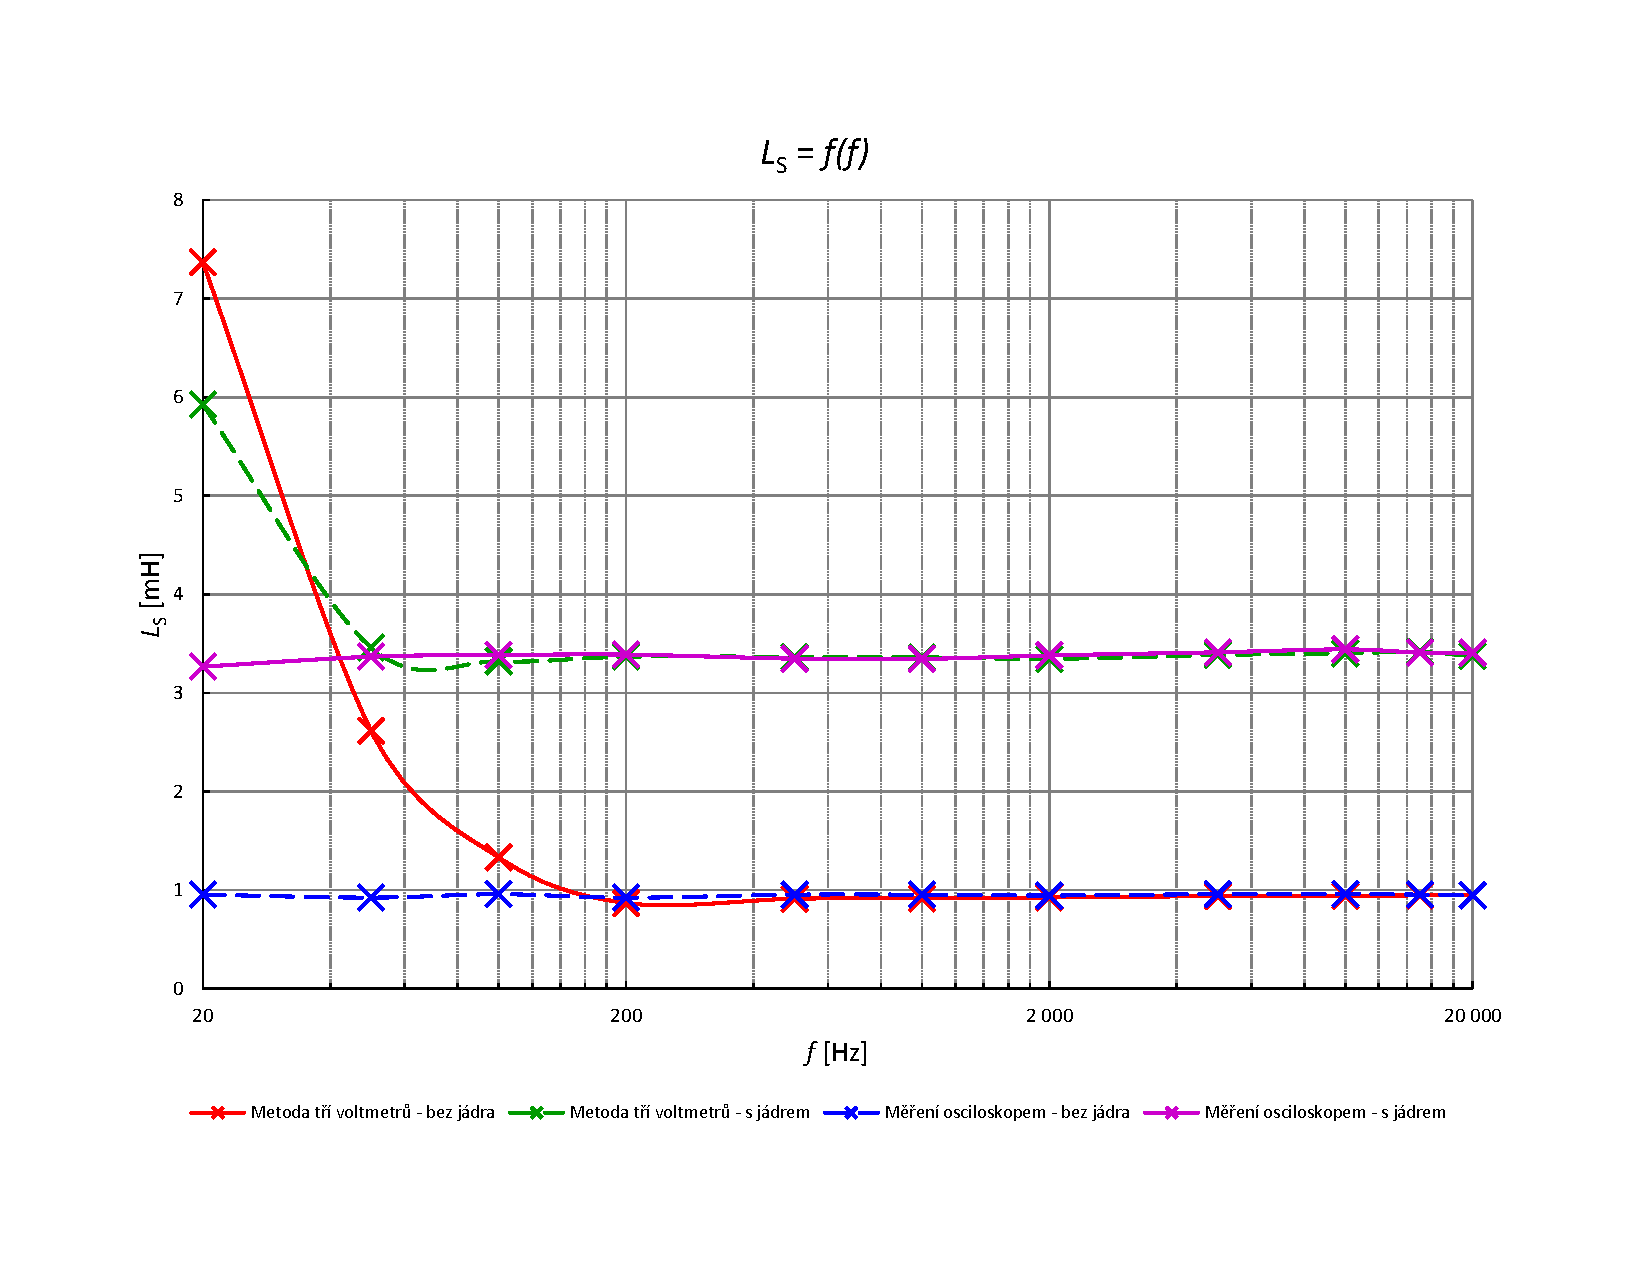
\includegraphics[width=\textwidth, trim={0 2.5cm 0 3cm}]{grafy/9B_graf1.pdf}
    \caption{Závislost indukčnosti cívky $L_\text{S}$ na kmitočtu $f$}
\end{figure}

\begin{figure}[H]
    \centering
    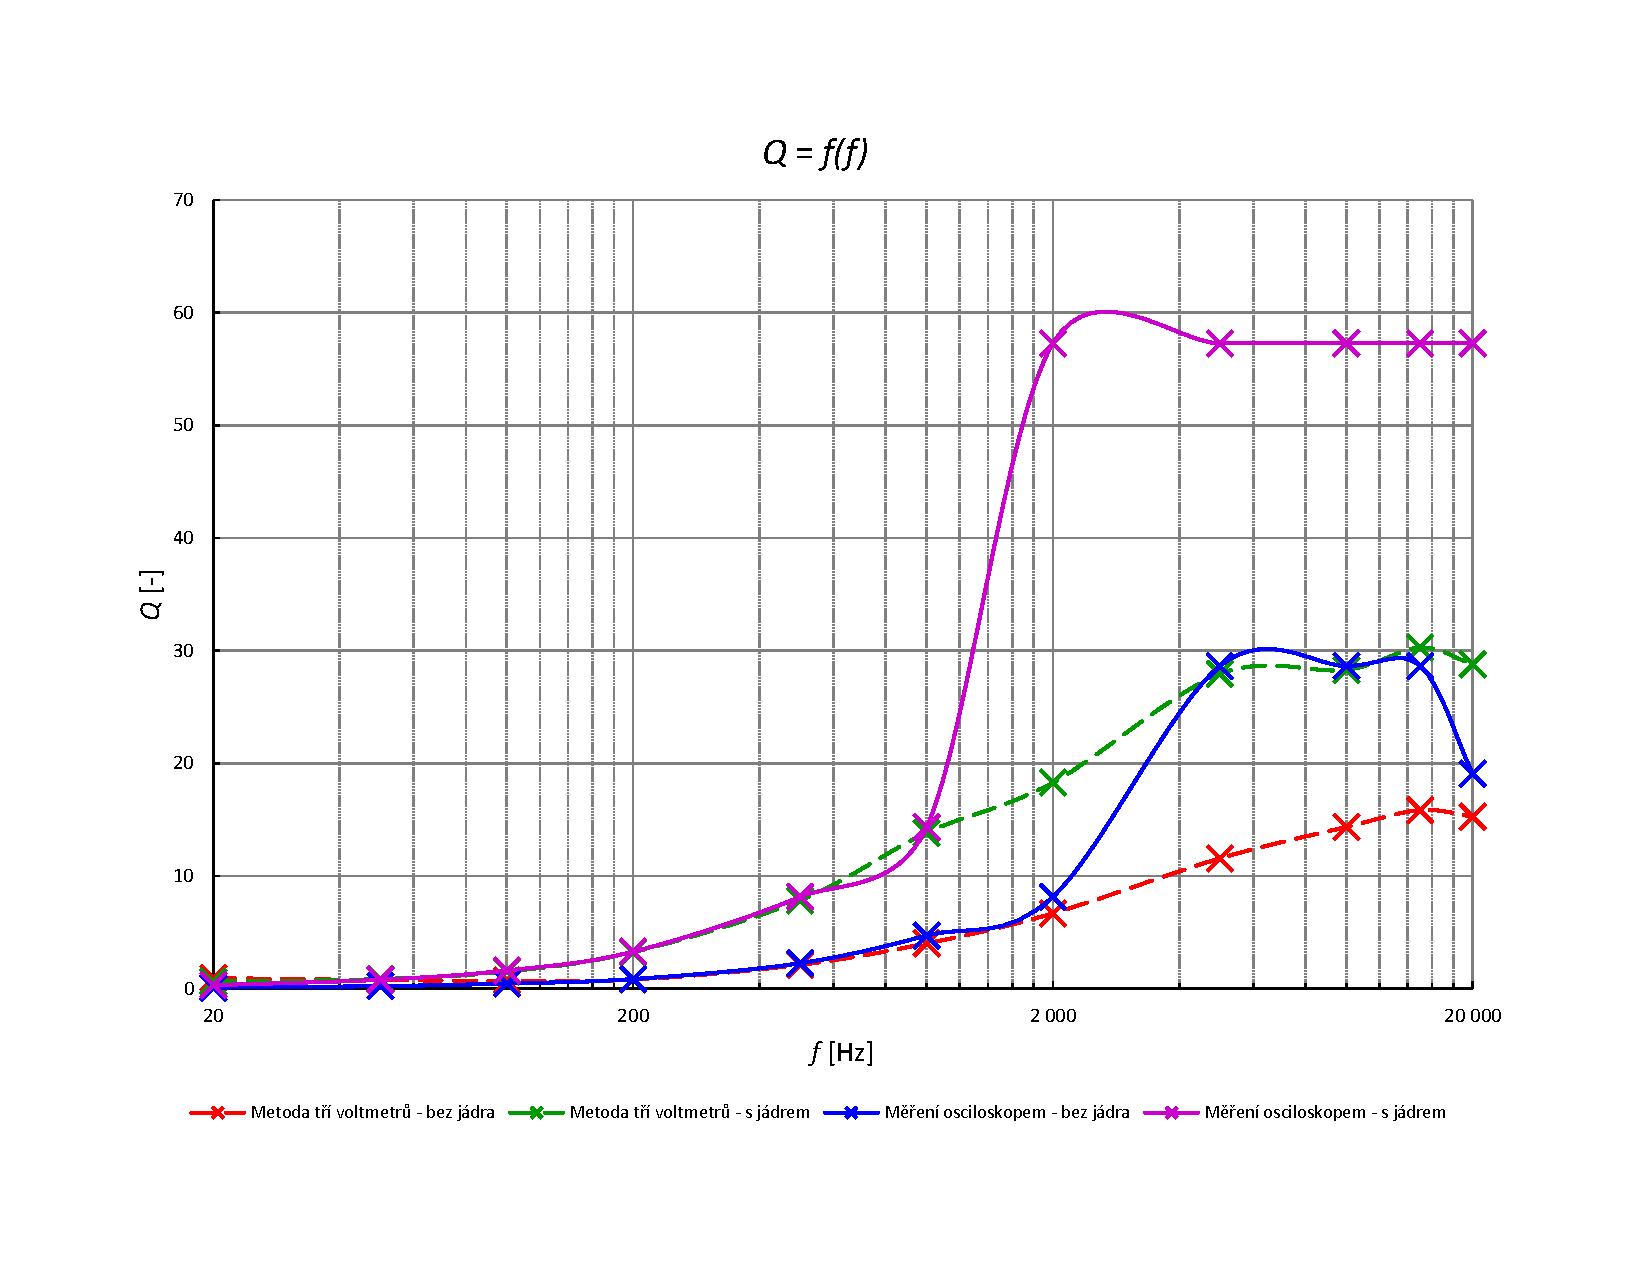
\includegraphics[width=\textwidth, trim={0 2.5cm 0 3cm}]{grafy/9B_graf2.pdf}
    \caption{Závislost činitele jakosti cívky $Q$ na kmitočtu $f$}
\end{figure}

\begin{figure}[H]
    \centering
    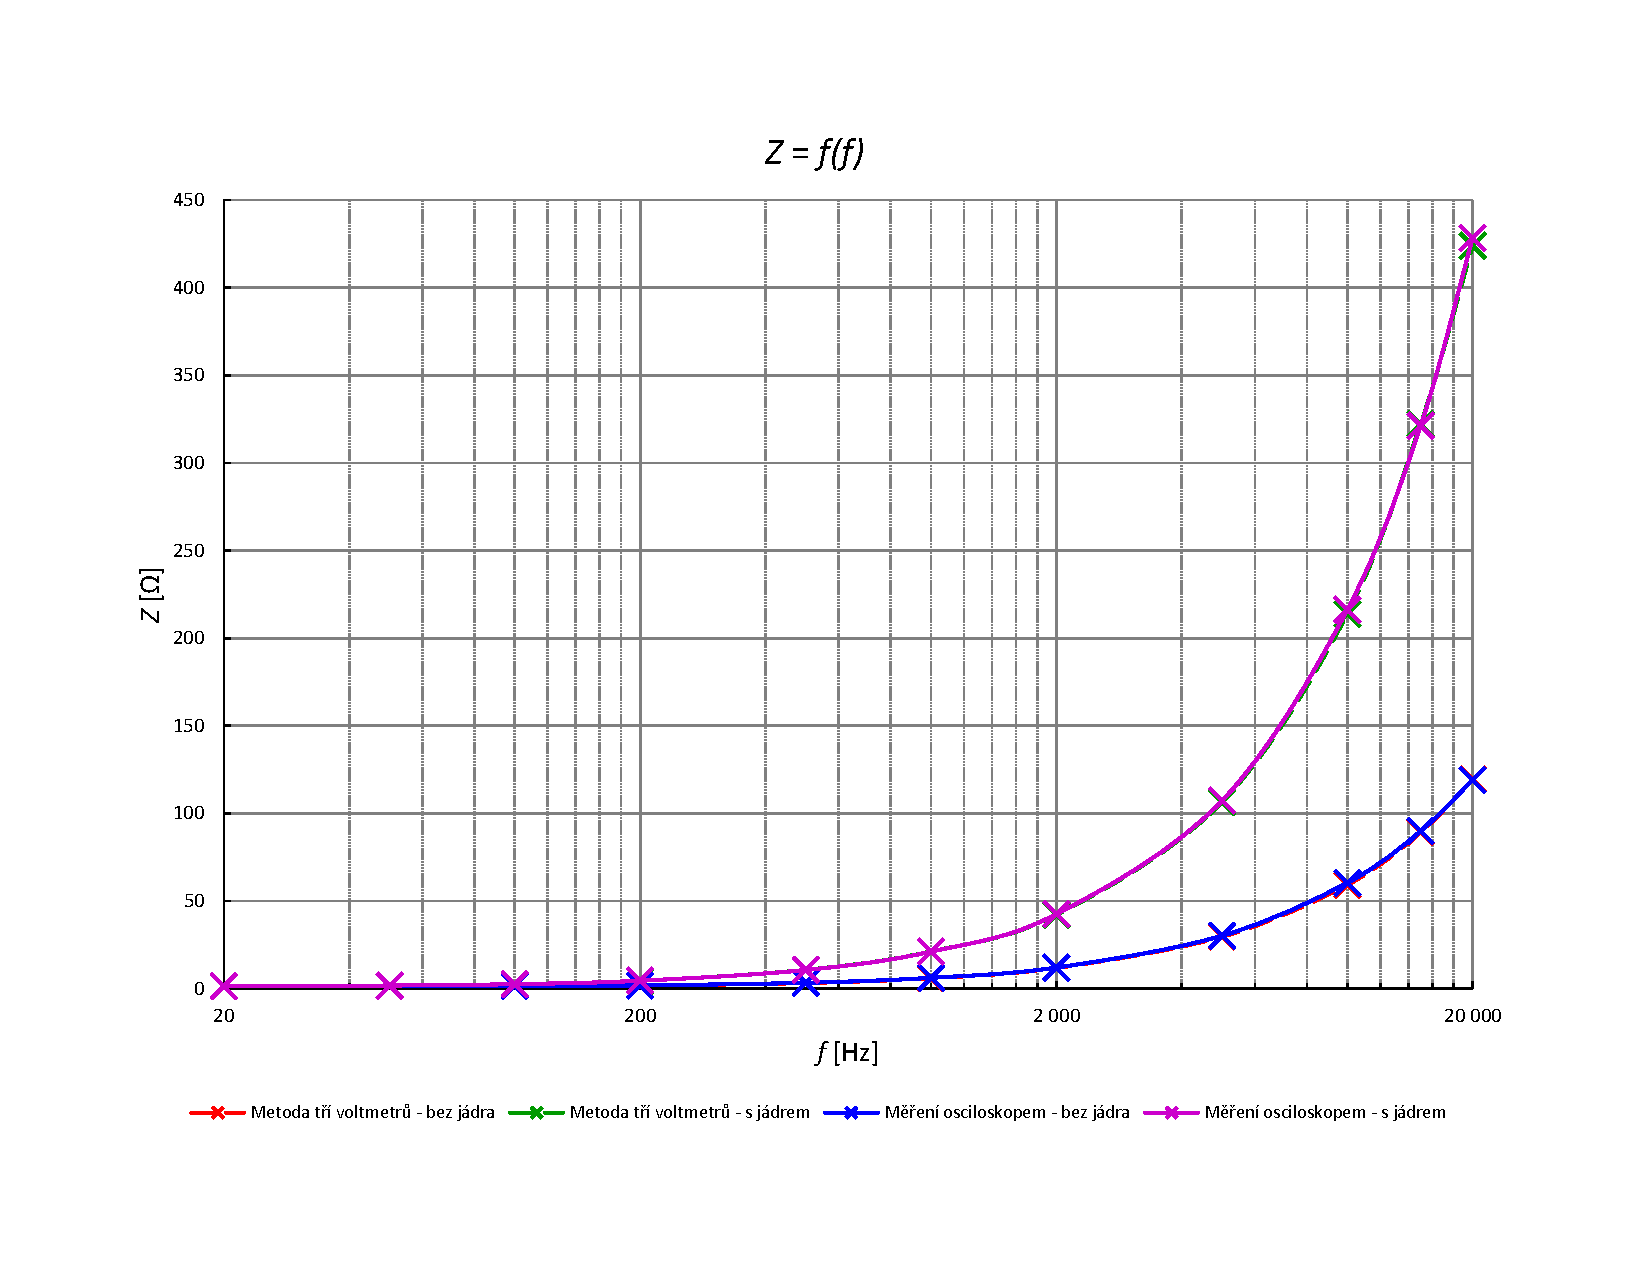
\includegraphics[width=\textwidth, trim={0 2.5cm 0 3cm}]{grafy/9B_graf3.pdf}
    \caption{Závislost impedance cívky $Z$ na kmitočtu $f$}
\end{figure}

\begin{figure}[H]
    \centering
    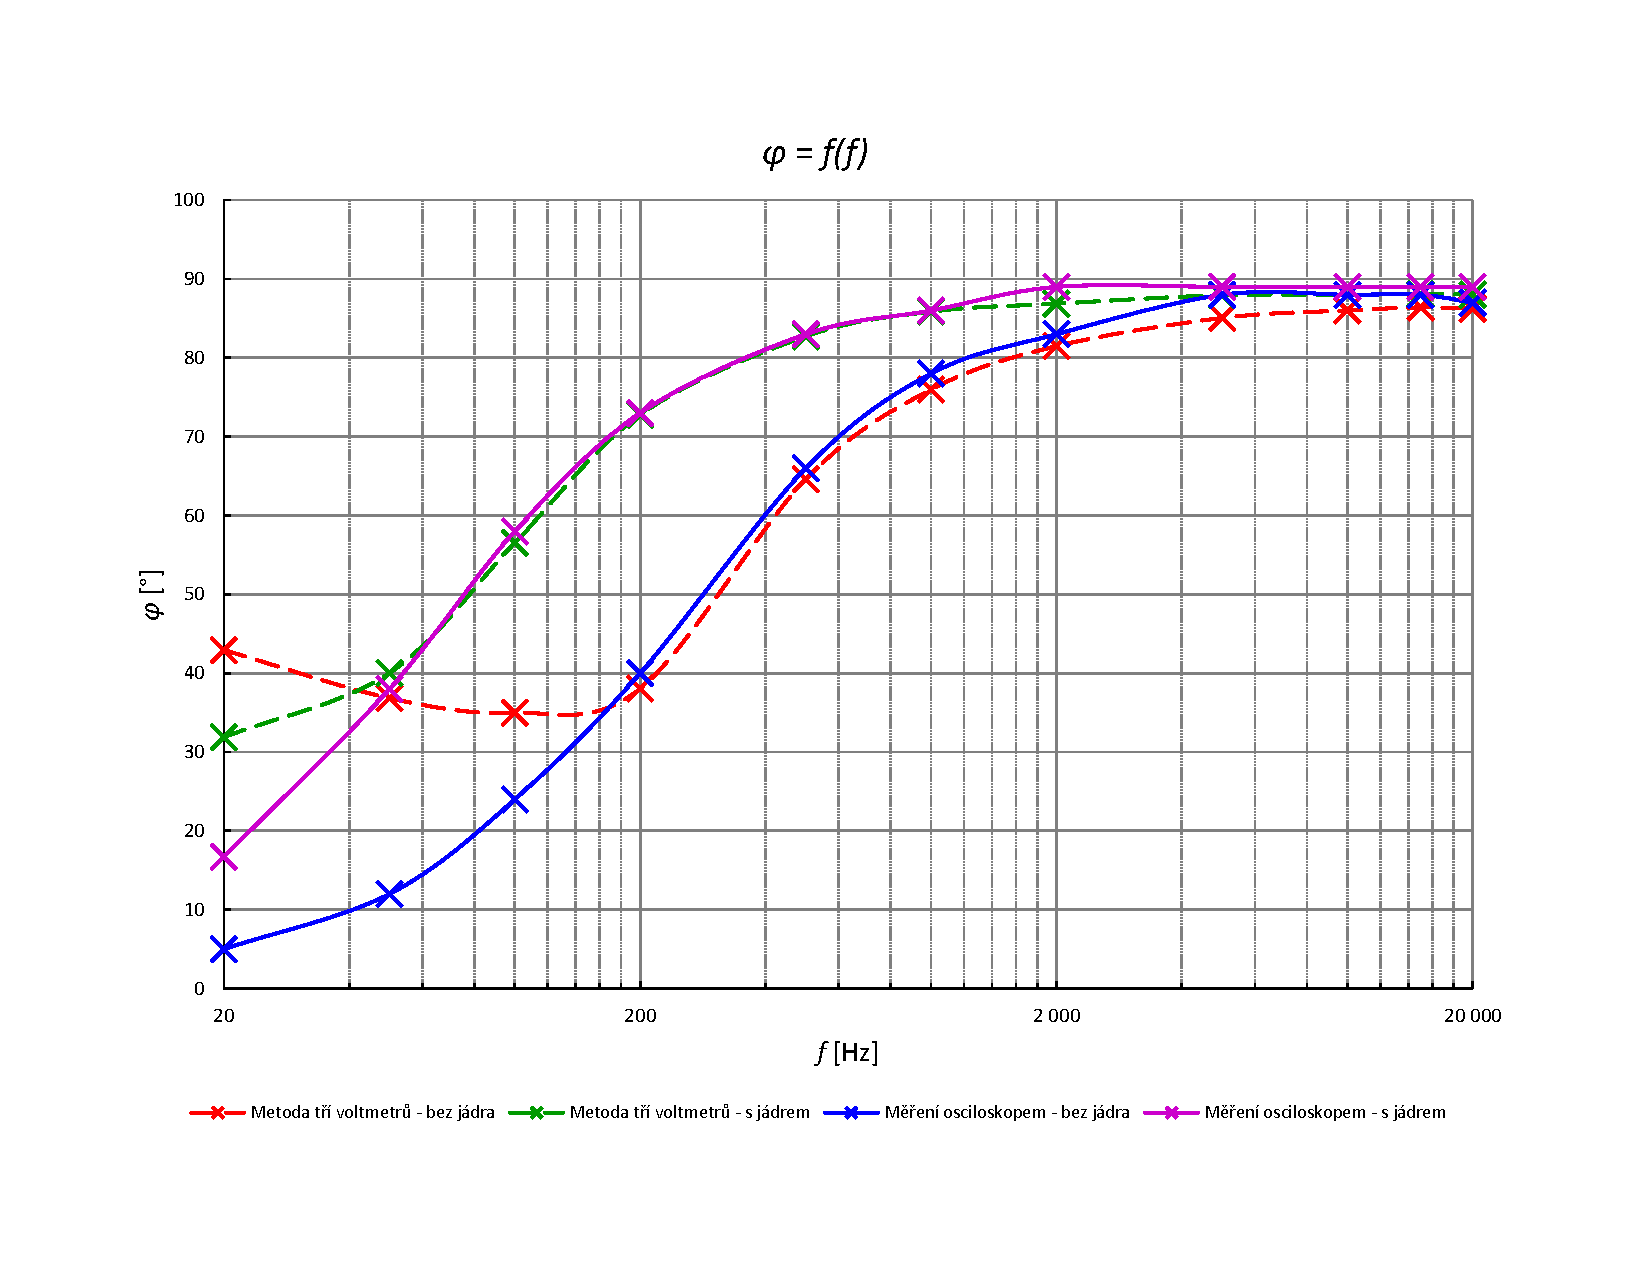
\includegraphics[width=\textwidth, trim={0 2.5cm 0 3cm}]{grafy/9B_graf4.pdf}
    \caption{Závislost fázového posunu cívky $\varphi$ na kmitočtu $f$}
\end{figure}

\subsection{Příklady výpočtu}

\begin{enumerate}
    \item Modul impedance
    \begin{multline*}
        Z = \textcolor{teal}{\frac{R \cdot U_Z}{U_R}} = \frac{100\,\Omega \cdot 13,6 \cdot 10^{-3}\,\text{V}}{1000 \cdot 10^{-3}\,\text{V}} = \underline{\underline{1,36\,\Omega}} \hfill
    \end{multline*}
    \item Fáze impedance
    \begin{multline*}
        \varphi = \textcolor{teal}{arcsin \left(\cfrac{\sqrt{4 U^2_R U^2_Z - \left(U^2 - U^2_R - U^2_Z\right)^2}}{2 U_R U_Z}\right)} = \hfill \\
        \ \ \ = arcsin \left(\cfrac{\sqrt{4 \cdot 1^2 \cdot (13,6 \cdot 10^{-3})^2 - \left((1010 \cdot 10^{-3})^2 - 1^2 - (13,6 \cdot 10^{-3})^2\right)^2}}{2 \cdot 1^2 \cdot 13,6 \cdot 10^{-3}}\right) =
        \underline{\underline{42,93\,\degree}} \hfill
    \end{multline*}
    \item Parametry náhradního obvodu měřené cívky
    \begin{multline*}
        R_\text{S} = \textcolor{teal}{Z \cdot cos\,\varphi} = 1,36\,\Omega \cdot cos (42,93\,\degree) = \underline{\underline{0,996\,\Omega}} \hfill \\
        \ \ \ L_\text{S} = \textcolor{teal}{\frac{Z \cdot sin\,\varphi}{2 \pi f}} = \frac{1,36\,\Omega \cdot sin(42,93\,\degree)}{2 \pi \cdot 20\,\text{Hz}} = \underline{\underline{7,371\,\text{mH}}} \hfill \\
        \ \ \ R_\text{P} = \textcolor{teal}{\frac{Z}{cos\,\varphi}} = \frac{1,36\,\Omega}{cos (42,93\,\degree)} = \underline{\underline{1,857\,\Omega}} \hfill \\
        \ \ \ L_\text{P} = \textcolor{teal}{\frac{1}{2 \pi f} \cdot \frac{Z}{sin\,\varphi}} = \frac{1}{2 \pi \cdot 20\,\text{Hz}} \cdot \frac{1,36\,\Omega}{sin(42,93\,\degree)} = \underline{\underline{15,89\,\text{mH}}} \hfill
    \end{multline*}
    \item Činitel jakosti
    \begin{multline*}
        Q = \textcolor{teal}{\frac{sin\,\varphi}{cos\,\varphi}} = \frac{sin(42,93\,\degree)}{cos(42,93\,\degree)} = \underline{\underline{0,93}} \hfill
    \end{multline*}
\end{enumerate}

\section{Seznam použitých přístrojů}

\section{Závěr}

\end{document}